
% This LaTeX was auto-generated from MATLAB code.
% To make changes, update the MATLAB code and republish this document.











    
    \begin{DoxyCode}
clear
\end{DoxyCode}
\begin{par}
COMPILATION
\end{par} \vspace{1em}
\begin{DoxyCode}
[exdir,~,~]=fileparts(which('example_model_5.m'));
% compile the model
amiwrap('model_example_5','example_model_5_syms',exdir)
\end{DoxyCode}

         \begin{DoxyCode}Generating model struct ...
Parsing model struct ...
Generating C code ...
headers | wrapfunctions | 
Compiling mex file ...
Building with 'Xcode with Clang'.
MEX completed successfully.
\end{DoxyCode} 
    \begin{par}
SIMULATION
\end{par} \vspace{1em}
\begin{DoxyCode}
% time vector
tout = linspace(0,4,9);
tfine = linspace(0,4,10001);
p = [1;0.4;2;3];
k = [];

D.Y = [  0.00714742903826096
      -0.00204966058299775
         0.382159034587845
          0.33298932672138
         0.226111476113441
         0.147028440865854
        0.0882468698791813
        0.0375887796628869
        0.0373422340295005];

D.Sigma_Y = 0.01*ones(size(D.Y));


options.sensi = 1;
options.sensi_meth = 'adjoint';
options.cvode_maxsteps = 1e4;
sol = simulate_model_example_5(tout,log10(p),k,D,options);
options.sensi = 0;
solfine = simulate_model_example_5(tfine,log10(p),k,[],options);

figure
errorbar(tout,D.Y,D.Sigma_Y)
hold on
plot(tfine,solfine.y)
legend('data','simulation')
xlabel('time t')
ylabel('observable')
title(['log-likelihood: ' num2str(sol.llh) ])
\end{DoxyCode}

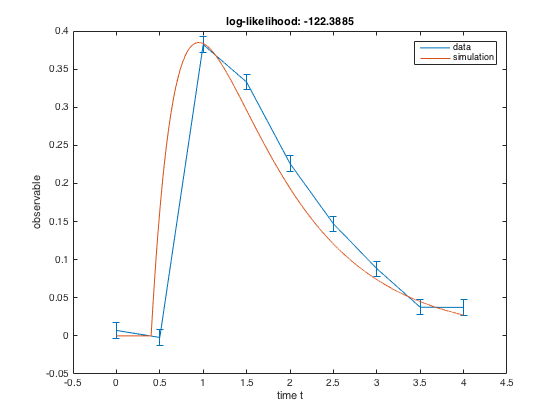
\includegraphics [width=4in]{../../examples/example_5/html/example_model_5_01.png}
\begin{par}
FD
\end{par} \vspace{1em}
\begin{DoxyCode}
eps = 1e-4;
xi = log10(p);
grad_fd_f = NaN(4,1);
grad_fd_b = NaN(4,1);
for ip = 1:4;
    options.sensi = 0;
    xip = xi;
    xip(ip) = xip(ip) + eps;
    solpf = simulate_model_example_5(tout,xip,k,D,options);
    grad_fd_f(ip,1) = (solpf.llh-sol.llh)/eps;
    xip = xi;
    xip(ip) = xip(ip) - eps;
    solpb = simulate_model_example_5(tout,xip,k,D,options);
    grad_fd_b(ip,1) = -(solpb.llh-sol.llh)/eps;
end

figure
plot(abs(grad_fd_f),abs(sol.sllh),'o')
hold on
plot(abs(grad_fd_b),abs(sol.sllh),'o')
set(gca,'XScale','log')
set(gca,'YScale','log')
hold on
axis square
plot([1e2,1e4],[1e2,1e4],'k:')
xlim([1e2,1e4])
ylim([1e2,1e4])
legend('forward FD','backward FD','Location','SouthEast')
xlabel('adjoint sensitivity absolute value of gradient element')
ylabel('computed absolute value of gradient element')
set(gcf,'Position',[100 300 1200 500])
\end{DoxyCode}

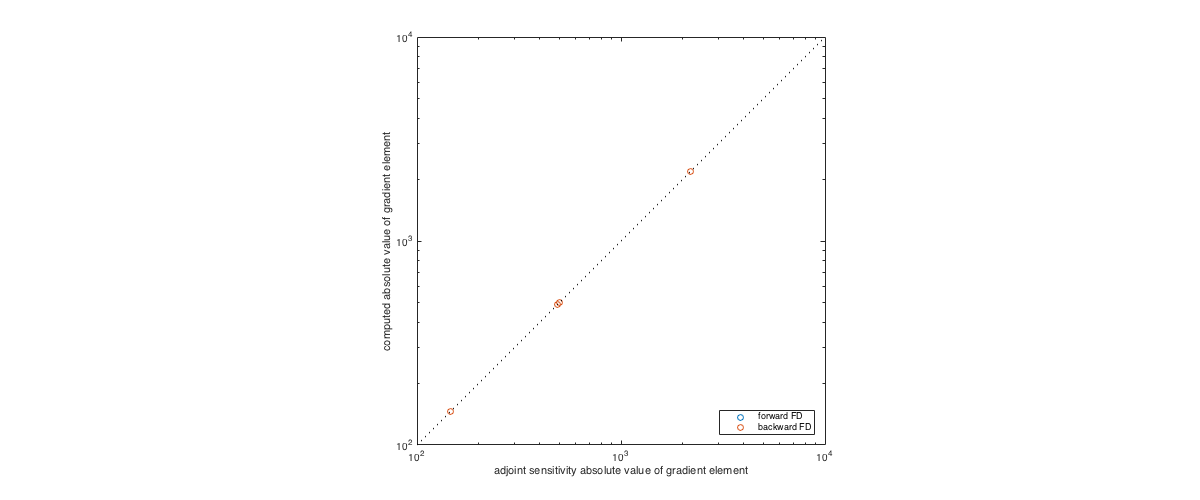
\includegraphics [width=4in]{../../examples/example_5/html/example_model_5_02.png}




    